\documentclass[a4paper]{article}
\usepackage[T1]{fontenc}
\usepackage[utf8]{inputenc}
\usepackage{tocloft,siunitx,amssymb,amsmath,graphicx,subcaption,float,pgf,pgfplots}
\usepackage[top=3cm,left=3cm,right=3cm]{geometry}
\graphicspath{{img/}}
\renewcommand\cftsecfont{\normalfont}
\renewcommand\cftsecpagefont{\normalfont}
\renewcommand{\cftsecleader}{\cftdotfill{\cftsecdotsep}}
\renewcommand\cftsecdotsep{\cftdot}
\renewcommand\cftsubsecdotsep{\cftdot}
\renewcommand\cftsubsubsecdotsep{\cftdot}
\title{Lab 2:Ohm's Law}
\author{
    Sebastián Nava López\\
    \and
    Ericka Sabrina Pensamiento R.\\
    \and
    Salvador Palos Gil
}
\captionsetup[subfigure]{justification=raggedright}
\begin{document}
\begin{titlepage}
    \centering
    {\Huge Instituto Politécnico Nacional}\\[3ex]
    {\huge Escuela Superior de Cómputo}\\[8ex]
    {\huge Fundamental Circuit Analysis}\\[12ex]
    {\Large Lab 2: Ohm's Law}\\[20ex]
    {\Large Group: 1CV7 Team: 7 \\[8ex]
    Sebastian Nava López\\[4ex]
    Sabrina Erika Pensamiento Robledo\\[4ex]
    Salvador Palos Gil\\[18ex]
    }
    \large{Elaboration: March 06,2018\hspace{8em} Due date: March 13,2018}
\end{titlepage}
\tableofcontents
\newpage
\section{Introduction}
As we know, OHM’S Law establishes that the potential difference ($V$) that we apply between the ends
of a given conductor is proportional to the intensity of the current ($I$) flowing through said conductor, completed the law introducing the notion of electrical resistance.
We will use a new element to do this practice as it is, a Potentiometer that is a three-terminal resistor with a sliding or rotating contact that forms an adjustable voltage divider. If only two terminals are used, one end and the wiper, it acts as a variable resistor.
The new concept we will understand in practice is Electric power that is the rate, per unit time, at which electrical energy is transferred by an electric circuit and unit of power is the watt, one joule per second.
Electric power, like mechanical power, is the rate of doing work, measured in watts, and represented
by the letter $P$. The term wattage is used colloquially to mean "electric power in watts." The
electric power in watts produced by an electric current $I$ consisting of a charge of $Q$ coulombs
every $t$ seconds passing through an electric potential (voltage) difference of $V$. Power is given
by:
\[P=VI\]\\
{\large{\textbf{Passive devices}}}\\ When electric charges move through a potential difference from a
higher to a lower voltage, that is when conventional current (positive charge) moves from the
positive ($+$) terminal to the negative ($-$) terminal, work is done by the charges on the device.
The potential energy of the charges due to the voltage between the terminals is converted to kinetic
energy in the device. These devices are called passive components or loads; they 'consume' electric
power from the circuit, converting it to other forms of energy such as mechanical work, heat, light,
etc.\\[2ex]
{\large{\textbf{Active devices or power sources}}}\\ If the charges are moved by an 'exterior force' through the device in the direction from the lower electric potential to the higher, (so positive charge moves from the negative to the positive terminal), work will be done on the charges, and energy is being converted to electric potential energy from some other type of energy, such as mechanical energy or chemical energy. Devices in which this occurs are called active devices or power sources; such as electric generators and batteries.
In this practice we will understand and manage the correct use of Ohm’s law trough analyzing what happens in the circuit with calculation support and experimentation. This way we'll understand the behavior of the current with respect to voltage and resistance.
\newpage
\section{Development}
\subsection{Voltage Dependence}
In the first part of the experiment we connected the $\SI{1}{\kilo\ohm}$ resistor,the
$\SI{2.5}{\kilo\ohm}$ potentiometer set at $\SI{2.5}{\kilo\ohm}$,an ammeter and the variable voltage supply in series
and then we measured the current from $\SI{0}{\volt}$ to $\SI{15}{\volt}$, increasing the
voltage $\SI{1}{\volt}$ at a time.
\subsubsection{Calculations}
Ohm's law states that:
\[I=\frac{V}{R}\]
where $V$ is voltage applied across the circuit measured in volts($\si{\volt}$), $I$ is the current flowing
through the circuit measured in amperes($\si{\ampere}$) and $R$ is the total resistance of the
circuit measured ohms($\si{\ohm}$).
Then, if $R_1=\SI{2.5}{\kilo\ohm}$ and $R_2=\SI{1}{\kilo\ohm}$, $R_{eq}$ is given by:
\begin{gather*}
    R_{eq}=R_1+R_2=\SI{2.5}{\kilo\ohm}+\SI{1}{\kilo\ohm}\\
    R_{eq}=\SI{3.5}{\kilo\ohm}
\end{gather*}
therefore, current is given by:
\[I_t=\frac{V}{R_{eq}}\]
for each voltage, we have:\\
%0v
$V=\SI{0}{\volt}$
\[I_t=\frac{\SI{0}{\volt}}{\SI{3.5}{\kilo\ohm}}=\SI{0}{\ampere}\]
%1v
$V=\SI{1}{\volt}$
\[I_t=\frac{\SI{1}{\volt}}{\SI{3.5}{\kilo\ohm}}=\SI{0.287}{\milli\ampere}\]
%2v
$V=\SI{2}{\volt}$
\[I_t=\frac{\SI{2}{\volt}}{\SI{3.5}{\kilo\ohm}}=\SI{0.571}{\milli\ampere}\]
%3v
$V=\SI{3}{\volt}$
\[I_t=\frac{\SI{3}{\volt}}{\SI{3.5}{\kilo\ohm}}=\SI{0.857}{\milli\ampere}\]
%4v
$V=\SI{4}{\volt}$
\[I_t=\frac{\SI{4}{\volt}}{\SI{3.5}{\kilo\ohm}}=\SI{1.143}{\milli\ampere}\]
%5v
$V=\SI{5}{\volt}$
\[I_t=\frac{\SI{5}{\volt}}{\SI{3.5}{\kilo\ohm}}=\SI{1.428}{\milli\ampere}\]
%6v
$V=\SI{6}{\volt}$
\[I_t=\frac{\SI{6}{\volt}}{\SI{3.5}{\kilo\ohm}}=\SI{1.714}{\milli\ampere}\]
%7v
$V=\SI{7}{\volt}$
\[I_t=\frac{\SI{7}{\volt}}{\SI{3.5}{\kilo\ohm}}=\SI{2.000}{\milli\ampere}\]
%8v
$V=\SI{8}{\volt}$
\[I_t=\frac{\SI{8}{\volt}}{\SI{3.5}{\kilo\ohm}}=\SI{2.286}{\milli\ampere}\]
%9v
$V=\SI{9}{\volt}$
\[I_t=\frac{\SI{9}{\volt}}{\SI{3.5}{\kilo\ohm}}=\SI{2.571}{\milli\ampere}\]
%10v
$V=\SI{10}{\volt}$
\[I_t=\frac{\SI{10}{\volt}}{\SI{3.5}{\kilo\ohm}}=\SI{2.857}{\milli\ampere}\]
%11v
$V=\SI{11}{\volt}$
\[I_t=\frac{\SI{11}{\volt}}{\SI{3.5}{\kilo\ohm}}=\SI{3.143}{\milli\ampere}\]
%12v
$V=\SI{12}{\volt}$
\[I_t=\frac{\SI{12}{\volt}}{\SI{3.5}{\kilo\ohm}}=\SI{3.428}{\ampere}\]
%13v
$V=\SI{13}{\volt}$
\[I_t=\frac{\SI{13}{\volt}}{\SI{3.5}{\kilo\ohm}}=\SI{3.714}{\ampere}\]
%14v
$V=\SI{14}{\volt}$
\[I_t=\frac{\SI{14}{\volt}}{\SI{3.5}{\kilo\ohm}}=\SI{4.000}{\ampere}\]
%15v
$V=\SI{15}{\volt}$
\[I_t=\frac{\SI{15}{\volt}}{\SI{3.5}{\kilo\ohm}}=\SI{4.286}{\ampere}\]
\subsubsection{Measurements}
\begin{center}
    \begin{tabular}{|c|c|c|}
        \hline
        Voltage Supply($\si{\volt}$) & Measured Current Value($\si{\milli\ampere}$) & Calculated
        Current Value($\si{\milli\ampere}$)\\\hline
        0&0&0\\\hline
        1&0.284&0.287\\\hline
        2&0.581&0.571\\\hline
        3&0.847&0.851\\\hline
        4&1.120&1.143\\\hline
        5&1.300&1.428\\\hline
        6&1.690&1.714\\\hline
        7&1.947&2.000\\\hline
        8&2.255&2.286\\\hline
        9&2.521&2.571\\\hline
        10&2.770&2.857\\\hline
        11&3.039&3.143\\\hline
        12&3.410&3.428\\\hline
        13&3.600&3.713\\\hline
        14&4.070&4.000\\\hline
        15&4.180&4.286\\\hline
    \end{tabular}
    %-----------------graph---------------
    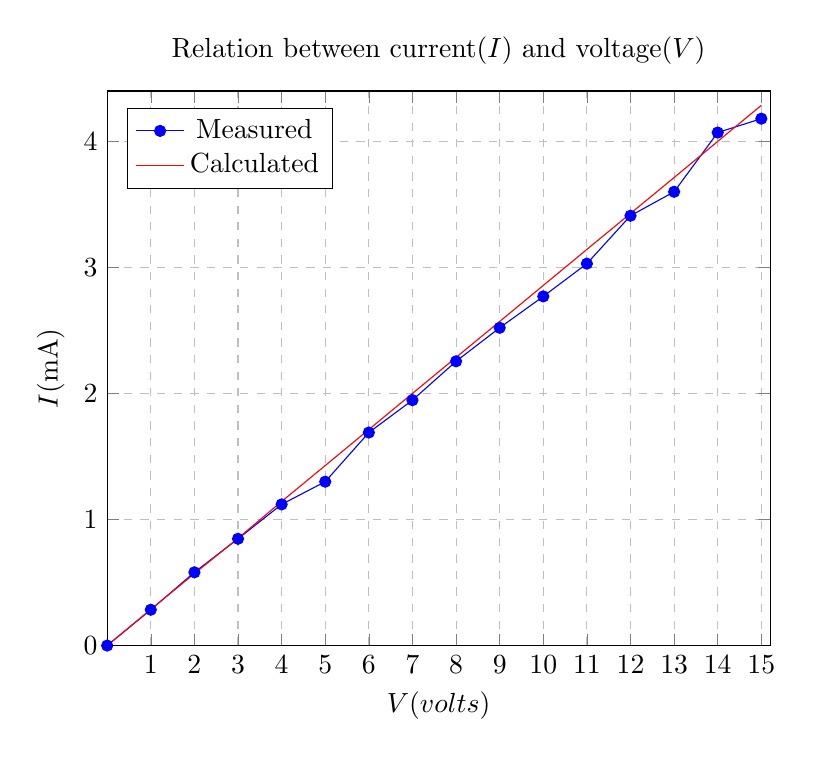
\begin{tikzpicture}
    \begin{axis}[
            title = {Relation between current($I$) and voltage($V$)},
            width=10cm,
            xlabel= {$V(volts)$},
            ylabel= {$I(\si{\milli\ampere})$},
            xmin=0,xmax=15.2,
            ymin=0,ymax=4.4,
            grid = both,
            xtick={1,2,...,15},
            grid style=dashed,
            legend pos=north west,
        ]
        \addplot[
            color=blue,
            mark=*,
        ]
            coordinates{(0,0)(1,0.284)(2,0.581)(3,0.847)
         (4,1.120)(5,1.300)(6,1.690)(7,1.947)(8,2.255)
                         (9,2.521)
                         (10,2.77)
                         (11,3.03)
                         (12,3.41)
                         (13,3.60)
                         (14,4.07)
                         (15,4.18)};
                         \addlegendentry{Measured}
        \addplot[
            mark=.,
            color=red,
        ]
            coordinates{(0,0)(1,0.287)(2,0.571)(3,0.851)
         (4,1.143)(5,1.428)(6,1.714)(7,2)(8,2.286)
                         (9,2.571)
                         (10,2.857)
                         (11,3.143)
                         (12,3.428)
                         (13,3.713)
                         (14,4)
                         (15,4.286)};
                         \addlegendentry{Calculated}
    \end{axis}         
\end{tikzpicture}      
 
    %-----------------graph---------------
\end{center}
\subsubsection{Simulations}
\begin{figure}[H]
    \begin{subfigure}{0.333\textwidth}
        \includegraphics[width=.9\linewidth]{amp0}
    \end{subfigure}
    \begin{subfigure}{0.333\textwidth}
        \includegraphics[width=.9\linewidth]{amp1}
    \end{subfigure}
    \begin{subfigure}{0.333\textwidth}
        \includegraphics[width=.9\linewidth]{amp2}
    \end{subfigure}
    \begin{subfigure}{0.333\textwidth}
        \includegraphics[width=.9\linewidth]{amp4}
    \end{subfigure}
    \begin{subfigure}{0.333\textwidth}
        \includegraphics[width=.9\linewidth]{amp5}
    \end{subfigure}
    \begin{subfigure}{0.333\textwidth}
        \includegraphics[width=.9\linewidth]{amp6}
    \end{subfigure}
    \begin{subfigure}{0.333\textwidth}
        \includegraphics[width=.9\linewidth]{amp7}
    \end{subfigure}
    \begin{subfigure}{0.333\textwidth}
        \includegraphics[width=.9\linewidth]{amp8}
    \end{subfigure}
    \begin{subfigure}{0.333\textwidth}
        \includegraphics[width=.9\linewidth]{amp9}
    \end{subfigure}
    \caption{Simulations for $V=\SI{0}{\volt}$ to $V=\SI{9}{\volt}$ }
    \label{fig:1}
\end{figure}
\begin{figure}[H]
    \begin{subfigure}{0.333\textwidth}
        \includegraphics[width=.9\linewidth]{amp10}
    \end{subfigure}
    \begin{subfigure}{0.333\textwidth}
        \includegraphics[width=.9\linewidth]{amp11}
    \end{subfigure}
    \begin{subfigure}{0.333\textwidth}
        \includegraphics[width=.9\linewidth]{amp12}
    \end{subfigure}
    \begin{subfigure}{0.333\textwidth}
        \includegraphics[width=.9\linewidth]{amp13}
    \end{subfigure}
    \begin{subfigure}{0.333\textwidth}
        \includegraphics[width=.9\linewidth]{amp14}
    \end{subfigure}
    \begin{subfigure}{0.333\textwidth}
        \includegraphics[width=.9\linewidth]{amp15}
    \end{subfigure}
    \caption{Simulations for $V=\SI{10}{\volt}$ to $V=\SI{15}{\volt}$ }
    \label{fig:2}
\end{figure}
\subsection{Resistance Dependence}
In the second part of the experiment, with the circuit wired in the same way as in the first
part, we fixed the voltage
supply to $\SI{15}{\volt}$ and then we increased the resistance value of the potentiometer from
$\SI{0}{\ohm}$ to $\SI{2.5}{\kilo\ohm}$, $\SI{250}{\ohm}$ at a time.
\subsubsection{Calculations}
If current is given by:
\[I_t=\frac{V}{R_{eq}}\]
and $R_{eq}$ is given by:
   \[R_{eq}=R_1+R_2=\SI{1}{\kilo\ohm}+R_{pot}\]
for each potentiometer setting we have:\\
%1
$R_{eq}=\SI{0}{\ohm}+\SI{1}{\kilo\ohm}=\SI{1.000}{\kilo\ohm}$
\[I_t=\frac{\SI{15}{\volt}}{\SI{1}{\kilo\ohm}}
=\SI{15.000}{\milli\ampere}\]
%2
$R_{eq}=\SI{250}{\ohm}+\SI{1}{\kilo\ohm}=\SI{1.250}{\kilo\ohm}$
\[I_t=\frac{\SI{15}{\volt}}{\SI{1.250}{\kilo\ohm}}
=\SI{12.000}{\milli\ampere}\]
%3
$R_{eq}=\SI{500}{\ohm}+\SI{1}{\kilo\ohm}=\SI{1.500}{\kilo\ohm}$
\[I_t=\frac{\SI{15}{\volt}}{\SI{1.500}{\kilo\ohm}}
=\SI{10.000}{\milli\ampere}\]
%4
$R_{eq}=\SI{750}{\ohm}+\SI{1}{\kilo\ohm}=\SI{1.750}{\kilo\ohm}$
\[I_t=\frac{\SI{15}{\volt}}{\SI{1.750}{\kilo\ohm}}
=\SI{8.571}{\milli\ampere}\]
%5
$R_{eq}=\SI{1}{\kilo\ohm}+\SI{1}{\kilo\ohm}=\SI{2.000}{\kilo\ohm}$
\[I_t=\frac{\SI{15}{\volt}}{\SI{2.000}{\kilo\ohm}}
=\SI{7.500}{\milli\ampere}\]
%6
$R_{eq}=\SI{1.250}{\kilo\ohm}+\SI{1}{\kilo\ohm}=\SI{2.250}{\kilo\ohm}$
\[I_t=\frac{\SI{15}{\volt}}{\SI{2.250}{\kilo\ohm}}
=\SI{6.667}{\milli\ampere}\]
%7
$R_{eq}=\SI{1.500}{\kilo\ohm}+\SI{1}{\kilo\ohm}=\SI{2.500}{\kilo\ohm}$
\[I_t=\frac{\SI{15}{\volt}}{\SI{2.500}{\kilo\ohm}}
=\SI{6.000}{\milli\ampere}\]
%8
$R_{eq}=\SI{1.750}{\kilo\ohm}+\SI{1}{\kilo\ohm}=\SI{2.750}{\kilo\ohm}$
\[I_t=\frac{\SI{15}{\volt}}{\SI{2.750}{\kilo\ohm}}
=\SI{5.454}{\milli\ampere}\]
%9
$R_{eq}=\SI{2.000}{\kilo\ohm}+\SI{1}{\kilo\ohm}=\SI{3.000}{\kilo\ohm}$
\[I_t=\frac{\SI{15}{\volt}}{\SI{3.000}{\kilo\ohm}}
=\SI{5.000}{\milli\ampere}\]
%10
$R_{eq}=\SI{2.250}{\kilo\ohm}+\SI{1}{\kilo\ohm}=\SI{3.250}{\kilo\ohm}$
\[I_t=\frac{\SI{15}{\volt}}{\SI{3.250}{\kilo\ohm}}
=\SI{4.615}{\milli\ampere}\]
%11
$R_{eq}=\SI{2.500}{\kilo\ohm}+\SI{1}{\kilo\ohm}=\SI{3.500}{\kilo\ohm}$
\[I_t=\frac{\SI{15}{\volt}}{\SI{3.500}{\kilo\ohm}}
=\SI{4.286}{\milli\ampere}\]
\subsubsection{Measurements}
\begin{center}
    \begin{tabular}{|c|c|c|c|}
        \hline
        Potentiometer Value($\si{\ohm}$) & Total Resistance Value
        & Measured Current & Calculated Current
        \\
         & [$R_{pot}+R_1$]($\si{\kilo\ohm}$) & Value($\si{\milli\ampere}$) & Value($\si{\milli\ampere}$)\\\hline
        0&0.860&15.250&15.000\\\hline
        250&1.210&11.780&12.000\\\hline
        500&1.360&11.229&10.000\\\hline
        750&1.606&9.198&8.571\\\hline
        1000&1.856&7.860&7.500\\\hline
        1250&2.123&7.120&6.667\\\hline
        1500&2.235&6.680&6.000\\\hline
        1750&2.603&5.667&5.454\\\hline
        2000&2.818&5.110&5.000\\\hline
        2250&3.146&4.657&4.615\\\hline
        2500&3.357&4.438&4.286\\\hline
    \end{tabular}
    %------graph----------
    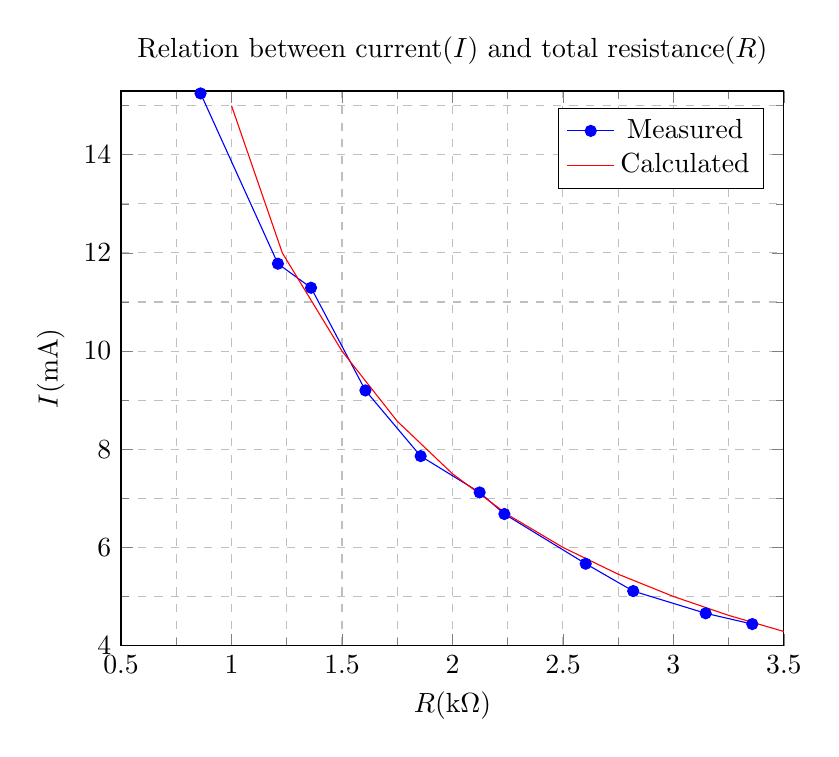
\begin{tikzpicture}
    \begin{axis}[
            title = {Relation between current($I$) and total resistance($R$)},
            width=10cm,
            xlabel= {$R(\si{\kilo\ohm})$},
            ylabel= {$I(\si{\milli\ampere})$},
            xmin=0.5,xmax=3.5,
            ymin=4,ymax=15.3,
            grid = both,
            minor tick num = 1,
            grid style=dashed,
            x tick label style={
                /pgf/number format/.cd,
                set decimal separator={$.$}
            },
            legend pos=north east,
        ]
        \addplot[
            color=blue,
            mark=*,
        ]
            coordinates{
(0.860,15.25)
(1.210,11.78)
(1.360,11.29)
(1.606,9.198)
(1.856,7.86)
(2.123,7.120)
(2.235,6.680)
(2.603,5.667)
(2.818,5.110)
(3.146,4.657)
(3.357,4.438)
                       };
                       \addlegendentry{Measured}
        \addplot[
            color=red,
            mark=,
        ]
            coordinates{
(1,15)
(1.23,12)
(1.5,10)
(1.75,8.571)
(2,7.5)
(2.25,6.667)
(2.5,6)
(2.75,5.454)
(3,5)
(3.25,4.615)
(3.5,4.286)
                       };
                       \addlegendentry{Calculated}
    \end{axis}         
\end{tikzpicture}      

    %------graph----------
\end{center}
\subsubsection{Simulations}
\begin{figure}[H]
    \begin{subfigure}{0.333\textwidth}
        \includegraphics[width=.9\linewidth,height=5.5cm]{pot0}
    \end{subfigure}
    \begin{subfigure}{0.333\textwidth}
        \includegraphics[width=.9\linewidth,height=5.5cm]{pot1}
    \end{subfigure}
    \begin{subfigure}{0.333\textwidth}
        \includegraphics[width=.9\linewidth,height=5.5cm]{pot2}
    \end{subfigure}
    \caption{Simulations for $R_{pot}=\SI{0}{\ohm}$ to $R_{pot}=\SI{500}{\ohm}$}
\end{figure}
\begin{figure}[H]
    \begin{subfigure}{0.333\textwidth}
        \includegraphics[width=.9\linewidth]{pot3}
    \end{subfigure}
    \begin{subfigure}{0.333\textwidth}
        \includegraphics[width=.9\linewidth]{pot4}
    \end{subfigure}
    \begin{subfigure}{0.333\textwidth}
        \includegraphics[width=.9\linewidth]{pot5}
    \end{subfigure}
    \begin{subfigure}{0.333\textwidth}
        \includegraphics[width=.9\linewidth]{pot6}
    \end{subfigure}
    \begin{subfigure}{0.333\textwidth}
        \includegraphics[width=.9\linewidth]{pot7}
    \end{subfigure}
    \begin{subfigure}{0.333\textwidth}
        \includegraphics[width=.9\linewidth]{pot8}
    \end{subfigure}
    \phantom{15em}
    \begin{subfigure}{0.333\textwidth}
        \includegraphics[width=.9\linewidth]{pot9}
    \end{subfigure}
    \hspace{.15\textwidth}
    \begin{subfigure}{0.333\textwidth}
        \includegraphics[width=.9\linewidth]{pot10}
    \end{subfigure}
    \caption{Simulations for $R_{pot}=\SI{750}{\ohm}$ to $R_{pot}=\SI{2500}{\ohm}$}
\end{figure}
\subsection{Power Measurement in Resistors}
In the last part we used two resistors, one $\SI{1}{\kilo\ohm}$, power rating \SI{1/4}{\watt}, and the other
$\SI{1}{\ohm}$, power rating \SI{1}{\watt}, we used each of them, in series with an ammeter and a voltage
supply fixed to $\SI{1}{\volt}$, to measure the current when connected.
\subsubsection{Calculations}
We know that current is:
\begin{equation}I=\frac{V}{R}\label{eq:ohms}\end{equation}
also, Power(P) is given by: 
\begin{equation}P=VI\label{eq:power}\end{equation}
substituting \ref{eq:ohms} in \ref{eq:power}, yields:
\begin{equation}P=\frac{V^2}{R}\label{eq:power2}\end{equation}
Then, for the $\SI{1}{\kilo\ohm}$ resistor, we have:
\[I=\frac{\SI{1}{\volt}}{\SI{1}{\kilo\ohm}}=\SI{1}{\milli\ampere}
\qquad P=\frac{(\SI{1}{\volt})^2}{\SI{1}{\kilo\ohm}}=\SI{1}{\milli\watt}\]
for the $\SI{1}{\ohm}$ resistor, we have:
\[I=\frac{\SI{1}{\volt}}{\SI{1}{\ohm}}=\SI{1}{\ampere}
\qquad P=\frac{(\SI{1}{\volt})^2}{\SI{1}{\ohm}}=\SI{1}{\watt}\]
If we look into the calculated power of the second resistor , we can see that the value is exactly the same
as the power rating of the resistor, so we are expecting the resistor to blow up when connected.
\subsubsection{Simulations}
\begin{figure}[H]
    \begin{subfigure}{0.40\textwidth}
        \includegraphics[width=.9\linewidth]{heat1}
    \caption{}
    \end{subfigure}
    \hspace{0.20\textwidth}
    \begin{subfigure}{0.40\textwidth}
        \includegraphics[width=.9\linewidth]{heat2}
    \caption{}
    \end{subfigure}
    \caption{Circuits using (a)\SI{1}{\kilo\ohm},\SI{1/2}{\watt} resistor and
    (b)\SI{1}{\ohm},\SI{1}{\watt} resistor }
\end{figure}
\section{Questions}
With the $\SI{1}{\kilo\ohm}$ resistor:\\[2ex]
\textit{What is the value of the current?
}:\\\phantom{3em}$I=\SI{0.910}{\milli\ampere}$\\ 
\textit{How much power is the resistor dissipating?}:\\\phantom{3em}$P=\SI{1/1000}{\watt}$\\ 
\textit{What was the effect on the resistor?}:\\\phantom{3em}There wasn't any visible effects\\ 
\textit{Why?}:\\\phantom{3em}Because the resistor can dissipate the heat caused by the voltage
drop\\
Then, using the $\SI{1}{\ohm}$ resistor:\\[2ex]
\textit{What is the value of the current?
}:\\\phantom{3em}$I=\SI{1.010}{\milli\ampere}$\\ 
\textit{How much power is the resistor dissipating?}:\\\phantom{3em}$P=\SI{1}{\watt}$\\ 
\textit{What was the effect on the resistor?}:\\\phantom{3em}Before we turned off the
voltage
source, the resistor started to smell burned and released white smoke\\ 
\textit{What's the difference between this circuit and the last one?}:\\\phantom{3em}The power
rating and the resistance value of the resistor used in this configuration is lower than the one used in the first
configuration\\
\textit{Why?}:\\\phantom{3em}Because the resistor couldn't handle the heat generated by the rate at which
electric charges are flowing trough the component\\

\section{Conclusions}
{\large Sabrina:}\\
For the engineer, it is vital to know Ohm's Law. Without it, there wouldn't be electricity at all. Therefore, the major importance of this law is that it allows us to enjoy the uses of our appliances now such as TV, refrigerator, Players, etc.
Ohm's law is also applied in circuit connections such as computing the power equation. With this, it
is easier to understand how to wire electrical components without the fear of low voltage or
electric shock.\\[2ex]
{\large Salvador:}\\
In this practice we understand the law of Ohm by making calculations of currents, voltages and resistances. In addition to understanding the behavior of the current with respect to voltage and resistance.\\[2ex]
{\large Sebastián:}\\
In the experiment we probed the relation between current, voltage and resistance in a circuit, learning that the current increases when there is a large voltage or there isn't great resistance in a circuit.Also we explore the use of a potentiometer to control the resistance value in a circuit. It's worth noting that in the second part of the experiment we experienced larger current values than the calculated ones because the $\SI{1}{\kilo\ohm}$ resistor just gave us a resistance of 860 ohm approximately, this can be attributed to a variety of factors involving the build quality or the handling of the component.
\end{document}
